\documentclass[a4paper,14pt]{extarticle}

\def\labauthors{Сарафанов Ф.Г., Платонова М.В.}
\def\labgroup{440}
\def\labnumber{1}
\def\labstartdate{5 ноября}
\def\labtheme{Измерение статических характеристик \\[0.2em] полевого транзистора}
\def\shortlabtheme{Полевой транзистор}

%!TEX root = ../fet.tex
\usepackage{cmap}
\usepackage[T2A]{fontenc}
\usepackage[utf8x]{inputenc}
\usepackage[english, russian]{babel}

\usepackage{misccorr} % в заголовках появляется точка, но при ссылке на них ее нет
\usepackage{amssymb,amsfonts,amsmath,amsthm}  
\usepackage{indentfirst}
\usepackage[usenames,dvipsnames]{color} 
\usepackage[unicode,hidelinks]{hyperref}
% \hypersetup{%
%     pdfborder = {0 0 0}
% }

\usepackage{makecell,multirow} 
\usepackage{ulem}
\usepackage{graphicx,wrapfig}
\graphicspath{{img/}}
\usepackage{geometry}
\geometry{left=2cm,right=2cm,top=3cm,bottom=3cm,bindingoffset=0cm,headheight=15pt}
\usepackage{fancyhdr} 
\linespread{1.05} 
\frenchspacing 
\renewcommand{\labelenumii}{\theenumii)} 
\newcommand{\mean}[1]{\langle#1\rangle}
% \usepackage{caption}
%%%%%%%%%%%%%%%%%%%%%%%%%%%%%%%%%%%%%%%%%%%%%%%%%%%%%%%%%%%%%%%%%%%%%%%%%%%%%%%
%%%%%%%%%%%%%%%%%%%%%%%%%%%%%%%%%%%%%%%%%%%%%%%%%%%%%%%%%%%%%%%%%%%%%%%%%%%%%%%



%%%%%%%%%%%%%%%%%%%%%%%%%%%%%%%%%%%%%%%%%%%%%%%%%%%%%%%%%%%%%%%%%%%%%%%%%%%%%%%
	%применим колонтитул к стилю страницы
\pagestyle{fancy} 
	%очистим "шапку" страницы
\fancyhead{} 
	%слева сверху на четных и справа на нечетных
\fancyhead[L]{\labauthors} 
	%справа сверху на четных и слева на нечетных
\fancyhead[R]{\shortlabtheme} 
	%очистим "подвал" страницы
\fancyfoot{} 
	% номер страницы в нижнем колинтуле в центре
\fancyfoot[C]{\thepage} 
\renewcommand{\phi}{\varphi}
%%%%%%%%%%%%%%%%%%%%%%%%%%%%%%%%%%%%%%%%%%%%%%%%%%%%%%%%%%%%%%%%%%%%%%%%%%%%%%%

\usepackage{float}
\usepackage[mode=buildnew]{standalone}
\usepackage{tikz} 
% \usepackage{subcaption}
\usepackage{csvsimple}
\usetikzlibrary{scopes}
\usetikzlibrary{%
     decorations.pathreplacing,%
     decorations.pathmorphing,%
    patterns,%
    calc,%
    scopes,%
    arrows,%
    % arrows.spaced,%
}
\makeatletter
\newif\if@gather@prefix 
\preto\place@tag@gather{% 
  \if@gather@prefix\iftagsleft@ 
    \kern-\gdisplaywidth@ 
    \rlap{\gather@prefix}% 
    \kern\gdisplaywidth@ 
  \fi\fi 
} 
\appto\place@tag@gather{% 
  \if@gather@prefix\iftagsleft@\else 
    \kern-\displaywidth 
    \rlap{\gather@prefix}% 
    \kern\displaywidth 
  \fi\fi 
  \global\@gather@prefixfalse 
} 
\preto\place@tag{% 
  \if@gather@prefix\iftagsleft@ 
    \kern-\gdisplaywidth@ 
    \rlap{\gather@prefix}% 
    \kern\displaywidth@ 
  \fi\fi 
} 
\appto\place@tag{% 
  \if@gather@prefix\iftagsleft@\else 
    \kern-\displaywidth 
    \rlap{\gather@prefix}% 
    \kern\displaywidth 
  \fi\fi 
  \global\@gather@prefixfalse 
} 
\newcommand*{\beforetext}[1]{% 
  \ifmeasuring@\else
  \gdef\gather@prefix{#1}% 
  \global\@gather@prefixtrue 
  \fi
} 
\makeatother

\usepackage{booktabs}
\usepackage{pgfplots, pgfplotstable}

\usepackage[outline]{contour}
\usepackage{tocloft}
\renewcommand{\cftsecleader}{\cftdotfill{\cftdotsep}} % for parts
% \renewcommand{\cftchapleader}{\cftdotfill{\cftdotsep}} % for chapters
\usepackage{pgfplots,pgfplotstable,booktabs,colortbl}
\pgfplotsset{compat=newest}
\usepackage{physics}
\usepackage{mathtools}
\mathtoolsset{showonlyrefs=true}
\newcommand\Smat{\hat { \mathbf { S } }}

\newcommand*\dotvec[1][1,1]{\crossproducttemp#1\relax}
\def\crossproducttemp#1,#2\relax{{\qty[\vec{#1}\times\vec{#2}\,]}}

\newcommand*\prodvec[1][1,1]{\crossproducttempa#1\relax}
\def\crossproducttempa#1,#2\relax{{\qty[{#1}\times{#2}\,]}}

% \def\E{\mathscr{E}_H}
\def\Rdim{\,\frac{\text{м}^3}{\text{А} \cdot \text{с}}}

\renewcommand{\vec}{\mathbf} % for parts
\begin{document}
%!TEX root = ../fet.tex
\begin{titlepage}
\begin{center}
% \vspace{-3em}
{\small\textsc{Нижегородский государственный университет имени Н.\,И. Лобачевского}}
\vskip 2pt \hrule \vskip 3pt
{\small\textsc{Радиофизический факультет}}

\vfill


{{\large Отчет по лабораторной работе №\labnumber}\vskip 12pt {\LARGE \bfseries \labtheme}}

	
\vspace{2cm}
{\large Работу выполнили студенты \\[-0.25em] \labgroup группы радиофизического факультата \\[0.5em] {\Large \bfseries \labauthors}}

% \vspace{0.5cm}
% {e-mail: sfg180@yandex.ru}

% \vspace{2cm}

\end{center}

\vfill
	
% \begin{flushright}
% 	{Выполнили студенты 430 группы\\ \labauthor}%\vskip 12pt Принял:\\ Менсов С.\,Н.}
% \end{flushright}
	
% \vfill
	
\begin{center}
	{Нижний Новгород, \labstartdate -- \today}
\end{center}

\end{titlepage}

\tableofcontents
\newpage



\addcontentsline{toc}{section}{Введение}
\section*{Введение}

В настоящей работе определяется  ы
с помощью ы-метода.  Как показано в \cite[стр. ы]{met}

\paragraph{Установка.} 
Все измерения базируются на получении  ы.
При измерениях снимаются показания ы.

\paragraph{Ы-метод.} 
Для реализации ы-метода используется ы.

Все измерения проводятся таким образом, чтобы ы.

\newpage

\section{Расчет ы}


\section{Теоретическое ы}


\newpage
\section{Экспериментальное ы}

\begin{figure}[h!]
    \centering
    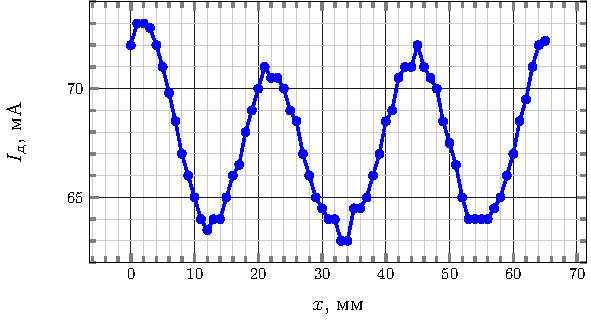
\includegraphics[scale=1.5]{fig/e2_from_x}
    \caption{Зависимость ы от  ы}
    \label{fig:exp:1}
\end{figure}




\addcontentsline{toc}{section}{Заключение}
\section*{Заключение}
В настоящей работе мы измерили ы.
Ы при ряде приближений ы.
Расхождение с практическими результатами объясняется ы.



\begin{thebibliography}{}
  \bibitem{orlov} Орлов И.\,Я., Односевцев В.\,А. и др. Основы радиоэлектроники: учебное пособие. -- Нижний Новгород: Нижегородский государственный университет им. Н.И. Лобачевского, 2011. -- 169 с.
  
  \bibitem{met} Битюрин\,\,Ю.\,А. и др. Измерение статических характеристик полевого транзистора. Н.Новгород: ННГУ, 2003. -- 30 с.
  
  % \bibitem{lit3} Ландау Л.Д., Лифшиц Е.М. Любой том. М.: Физматлит, 2003.
\end{thebibliography}

\end{document}